\chapter{Optical receivers}
\section{Introduction}
\begin{wrapfigure}[8]{r}{8cm}
\vspace{-5mm}
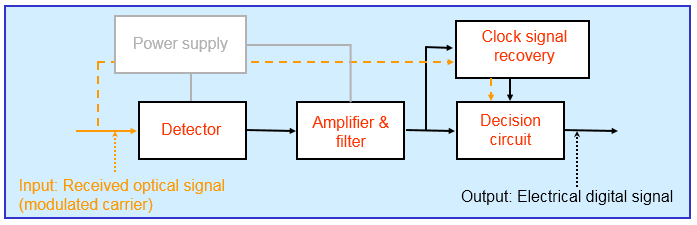
\includegraphics[scale=0.5]{ch5/image1}
\captionof{figure}{ }
\end{wrapfigure}
Le rôle d'un récepteur optique est de convertir un flux optique en un signal électrique puis de le
traiter afin de générer un flux de bits. Le premier élément est le bloc récepteur, constitué d'un
photo-détecteur semi-conducteur (photodiode $pn$, APD) puis d'un amplificateur (avec contrôle de 
gain automatique) et d'un filtre.  La dernière partie est le circuit de décision qui converti le 
signal analogique en une série de bits.

\section{Semiconductor photodiode}
\subsection{$p-n$ photodiode: source of photocurrent}
Le principe physique est la génération de porteurs libres par absorption de photons dans la zone
de charge d'espace d'une jonction $pn$, polarisée en inverse. En effet, si l'on prend du Si pur,
aucun courant ne circulera si l'on éclaire la jonction. Il y aura bien absorption, un peu de 
diffusion puis une recombinaison : il est nécessaire de polariser la jonction sans quoi ça n'ira pas.\\

Pour avoir de l'absorption, la condition suivante doit être remplie
\begin{equation}
{E_{photon}} = h\nu  = hc/\lambda  > {E_g}
\end{equation}
La génération du photo-courant se fait en trois étapes
\begin{enumerate}
\item Absorption d'un photon dans la zone de déplétion
\item Création d'une paire $e^-/h^+$
\item Dérive de ces charges libres par application d'un champ électrique : génère $I_p$
\end{enumerate}


\subsection{Photocurrent and Responsivity}
\begin{wrapfigure}[7]{l}{9cm}
\vspace{-5mm}
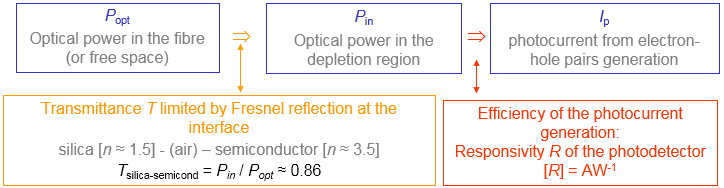
\includegraphics[scale=0.45]{ch5/image2}
\captionof{figure}{ }
\end{wrapfigure}
La \textbf{responsivity} d'une photodiode $R$ [A.W$^{-1}$] est le coefficient qui relie la 
puissance optique d'entrée $P_{in}$ [W] au photocourant $I_p$ [A]
\begin{equation}
{I_p} = R{P_{in}}
\end{equation}
 
\newpage
Celle-ci dépend de la longueur d'onde $\lambda$ et peut être liée à l'efficacité quantique $\eta$
de la photodiode. Ce-dernier est le rendement de la conversion d'un photon d'entrée en une paire
$e^-/h^+$
\begin{equation}
\eta  \buildrel \Delta \over = \frac{{\text{electron generation rate}}}{{\text{incident photon rate}}} = \frac{{{{{I_p}} \mathord{\left/
 {\vphantom {{{I_p}} q}} \right.
 \kern-\nulldelimiterspace} q}}}{{{{{P_{in}}} \mathord{\left/
 {\vphantom {{{P_{in}}} {h\nu }}} \right.
 \kern-\nulldelimiterspace} {h\nu }}}} = \frac{{h\nu }}{q}R
\end{equation}
La relation suivante montre que le courant est plus important lorsque la longueur d'onde augmente
\begin{equation}
\frac{R}{{(1\;A/W)}} = \eta \frac{1}{{(1\;A/W)}}\frac{{\rm{q}}}{{{\rm{h}}\nu }} = \eta \frac{1}{{(1\;A/W)}}\frac{{\rm{q}}}{{{\rm{h}}c}}\lambda  = \frac{\eta }{{1.24}}\;\;\frac{\lambda }{{(1\;\mu m)}}
\end{equation}
Soit une puissance constante. Si la longueur d'onde augmente, les photons sont moins énergétiques :
il faut un flux plus important pour maintenir la réponse constante. Comme un photon génère une paire, 
le courant sera plus important, d'où l'augmentation de $R$.

\subsubsection{Link between the absorption coefficient $\alpha$ in the depletion region and $\eta$}
\begin{wrapfigure}[8]{l}{5cm}
\vspace{-5mm}
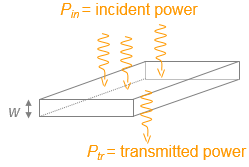
\includegraphics[scale=0.65]{ch5/image3}
\captionof{figure}{ }
\end{wrapfigure}
La puissance absorbée dans le SC dépend de $\alpha$ et de son épaisseur $w$, selon Beer-Lambert. La
puissance transmise vaut donc ${P_{tr}} = {P_{in}}\exp [ - \alpha .w]$. Donc, la puissance
absorbée
\begin{equation}
{P_{abs}} = {P_{in}} - {P_{tr}} = {P_{in}}(1 - \exp [ - \alpha .w])
\end{equation}
Si un photon absorbé $\to$ une paire $e^-/h^+$, l'efficacité quantique est donnée par
\begin{equation}
\eta  = \frac{{{P_{abs}}}}{{{P_{in}}}} = 1 - \exp [ - \alpha .w]
\end{equation}

\begin{wrapfigure}[12]{r}{7cm}
\vspace{-5mm}
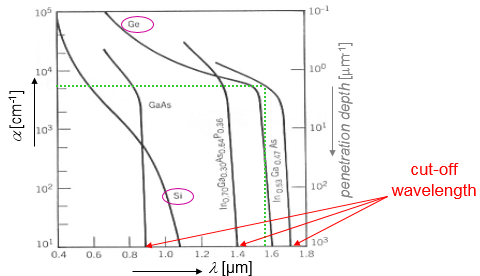
\includegraphics[scale=0.65]{ch5/image4}
\captionof{figure}{ }
\end{wrapfigure}
Ci-contre, l'évolution de $\alpha$ en fonction de $\lambda$. On peut voir qu'ici, contrairement aux
sources, on peut utiliser des SC à gap indirect comme le $Si$ et $Ge$ (les transitions indirectes de
la bande de valence à la bande de conduction sont possibles). Cependant,  en dessous de l'énergie de
la bande interdite directe, l'absorption des matériaux à bande interdite indirecte est moins efficace,
mais elle peut être compensée par une couche d'absorption plus épaisse.\\

Une énergie minimal est nécessaire pour générer une paire $e^-/h^+$ : $\alpha$ chute rapidement 
pour des énergies de photon inférieure à l'énergie de bande interdite, c'est-à-dire pour des 
longueur d'ondes supérieurs à celle de coupure. Toutes les photodiodes ne sont donc pas adaptées
à toutes les applications : le Si ne convient pas autour de 1.3 ou 1.5 nm.

\newpage
\subsection{$p-i-n$ Photodiode}
\begin{wrapfigure}[10]{l}{11cm}
\vspace{-5mm}
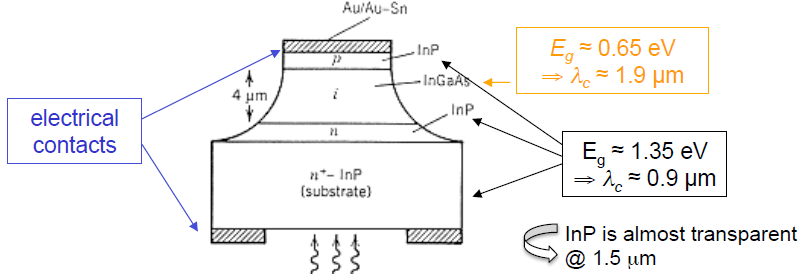
\includegraphics[scale=0.5]{ch5/image5}
\captionof{figure}{ }
\end{wrapfigure}
La plus simple des photodiodes est une jonction $pn$ polarisée en inverse : les photons absorbés
créent des paires $e^-/h^+$ qui, sous l'application du champ électrique créé par la tension, vont
générer le photo-courant (les électrons dérivent dans le côté $n$ et les trous dans le côté $p$). 
En dehors de la zone de déplétion, le champ électrique est faible et les charges créés dans ces
régions vont lentement migrer. Il en résulte un courant de dérive "lent" (bien plus lent que le 
temps de dérive dans la zone de charge d'espace) augmentant le temps de réponse de la photodiode :
limitation de la bande passante.\\

On peut s'arranger pour que le photon ne soit pas arrangé dans la bande $p$ et $n$, mais dans
une région intrinsèque qui possède un gap inférieure à l'énergie des photons (ce qui n'est pas
le cas des régions $p$ et $n$). On est alors en possession d'une région intrinsèque de grande
résistivité sur laquelle on peut appliquer une grande tension. De plus, comme il n'y a pas de 
courant de diffusion, la bande passante est plus importante. Ce dispositif est une photodiode
$p-i-n$. En résumé, trois avantages
\begin{enumerate}
\item Pas de courant de diffusion $\to$ bande passante plus importante
\item Épaisseur de la couche d'absorption (intrinsèque) plus facilement contrôlabl
\item Augmentation de l'efficacité quantique (car pas d'absorption en dehors de la zone $i$)
\end{enumerate}


\subsection{Avanlanche photodiode (APD)}
Dans une photodiode $p-n$ ou $p-i-n$, le photo-courant est donné par
\begin{equation}
{I_p} = R{P_{in}} \le \frac{q}{{h\nu }}{P_{in}}
\end{equation}
Il est limité par le nombre de photons incident qui produit une paire $e^-/h^+$. Dans une
\textbf{photodiode à avalanche}, celui-ci est amplifié grâce à une responsivity $R>q/h\nu$.\\

\begin{wrapfigure}[10]{r}{6cm}
\vspace{-5mm}
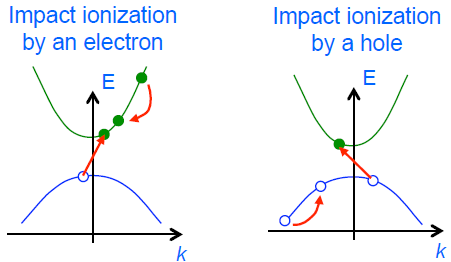
\includegraphics[scale=0.5]{ch5/image6}
\captionof{figure}{Perte d'énergie de la charge accélérée (courbe) : génération paire (droit) }
\end{wrapfigure}
L'amplification se fait par ionisation d'impact : une charge libre est accélérée par un grand
champ électrique ($\approx10^5$ V/cm) qui augmente l'énergie de la charge. Si elle est 
assez grande, une partie de cette énergie cinétique peut être transférée à un électron lié qui
va aller dans la bande de valence (collision) : nouvelle paire produite qui contribue au 
photo-courant. Celle-ci peut aussi être accélérée et produire d'autres paires. Dès lors, un photon
absorbé va donner $M$ paires $e^-/h^+$\footnote{Haute énergie veut dire "haut" dans la bande de 
valence et "bas" dans la bande de conduction.}.\\

\begin{wrapfigure}[4]{r}{4cm}
\vspace{-5mm}
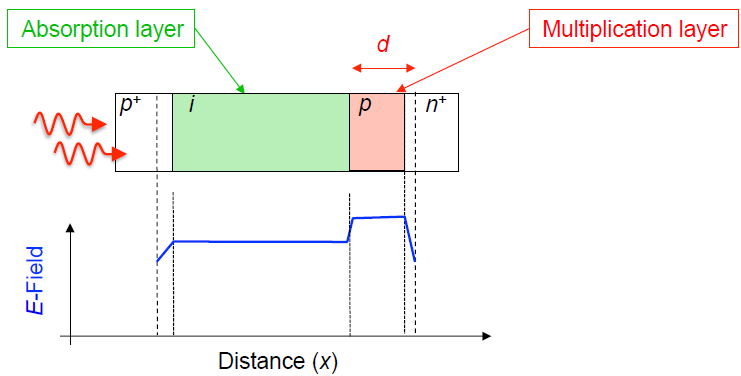
\includegraphics[scale=0.25]{ch5/image7}
\captionof{figure}{ }
\end{wrapfigure}
D'un point de vue pratique, on évite d'avoir une $p-i-n$ avec de l'avalanche dans $i$. On préfère
avoir deux régions spatiales : un où on amplifie et l'autre où on absorbe (zone $d$). On parle
 d'\textbf{APD}. Ceci permet un meilleur contrôle du facteur d'amplification $M$.
 
\subsubsection{Calculation of the current gain}
On peut calculer ce gain grâce à des équations de bilan. On sait que le taux d'amplification du
courant dépend du \textit{impact-ionization coefficient} des électrons $\alpha_e$ et des
trous $\alpha_h$. Soit $i_e$ le courant d'électrons $i_h$ le courant de trous. On en tire
\begin{equation}
\left\{\begin{array}{ll}
\DS\frac{{d{i_e}}}{{dx}} &\DS= {\alpha _e}{i_e} + {\alpha _h}{i_h}\vspace{2mm}\\
\frac{{d{i_e}}}{{dx}} &\DS= {\alpha _e}{i_e} + {\alpha _h}{i_h}
\end{array}\right.
\end{equation}
Pour le courant lié aux électrons, ceux-ci contribuent mais les trous également. Le courant de 
trous, lui, se déplace dans l'autre sens. On remarque rapidement que le courant total 
$I=i_e(x)+i_h(x)$ est constant dans la couche de multiplication. Notons que les coefficients 
$\alpha_i$ dépendent du matériel \textbf{et} du champ électrique dans cette même zone.

\subsubsection{Multiplication factor($M$)}
Le but de la séparation des couches est de savoir quelle espèce entre dans la région de 
multiplication, ce qui permet de contrôler $M$. A partir des deux précédentes équations de bilan, 
on peut en obtenir une seule pour l'évolution du courant des électrons libre en fonction de la
position $x$ dans la couche d'amplification.
\begin{equation}
\frac{{d{i_e}}}{{dx}} = ({\alpha _e} - {\alpha _h}){i_e} + {\alpha _h}I
\end{equation}
Faisons deux hypothèses
\begin{enumerate}
\item Le champ électrique dans la couche de multiplication est uniforme : $\alpha_i$ constants et
$\alpha_e>\alpha_h$.
\item On ne considère ici que les électrons dans la couche de multiplication. 
\begin{itemize}
\item Ceci donne les CL : $i_h(d)=0$ (pas de trous), $i_e(d)=I$.
\end{itemize}
\end{enumerate}
Après résolution
\begin{equation}
{i_e}(0) = \frac{{I\exp ( - {\alpha _e}[1 - {k_a}]d)}}{{1 - {k_a}}} - \frac{{{k_a}I}}{{1 - {k_a}}}
\end{equation}
où $k_a = \alpha_h/\alpha_e$. On en tire une valeur moyenne du gain d'amplification $M$
 (l'amplification n'est pas identique à chaque fois)
\begin{equation}
M = \frac{I}{{{i_e}(0)}} = \frac{{1 - {k_a}}}{{\exp ( - {\alpha _e}[1 - {k_a}]d) - {k_a}}}
\end{equation}
La responsivity d'une photodiode APD est donc $M$ fois la responsivity d'une photodiode $p-i-n$ 
qui possède la même couche d'absorption
\begin{equation}
{R_{{\rm{APD}}}} = MR = M\eta \frac{q}{{h\nu }}
\end{equation}
On peut voir que $M$ dépend fortement des \textit{impact ionization coefficient}
\begin{equation}
\alpha_h\ll \alpha_e\quad\Rightarrow\quad M{\rm{ }} \approx {\rm{ exp( + }}{\alpha _e}d)\qquad\qquad
\alpha_h\approx \alpha_e\quad\Rightarrow\quad M{\rm{ }} \approx {\rm{ }}1/(1 - {\alpha _e}d)
\end{equation}
Comme ceux-ci dépendent du champ électrique, on peut contrôler $M$ à travers la tension appliquée.
Comme les électrons et les trous jouent un rôle égal, il y a un risque de claquage par avalanche 
lorsque $\alpha_ed=1 \to M=\infty$. Pour cette raison, on utilisera un matériau tel que seulement
les trous \textbf{ou} les électrons provoquent des avalanches\footnote{Ceci a cependant de 
l'intérêt pour la détection de photons uniques.}

\subsubsection{Bande passante de l'APD}
L'inconvénient de l'APD est le temps de transition requis pour la génération et la collection 
des paires secondaires : le gain va dépendre de la fréquence à cause de ce temps de transition
\begin{equation}
M(\omega ) = \frac{{{M_0}}}{{\sqrt {1 + {{[\omega {\tau _e}{M_0}]}^2}} }}
\end{equation}
La bande passante vaut alors $\Delta f{\rm{  =  }}\sqrt 3 {\rm{/(}}2\pi {\tau _e}{M_0})$. Il 
faudra donc faire un compromis entre un APD sensible (grand $M$) et la bande passante (petit $M$).

\section{Receiver: beyond the detector}
\subsection{Architecture of a digital optical receiver (amplitude modulation \& direct detection)}
\begin{wrapfigure}[4]{r}{4cm}
\vspace{-5mm}
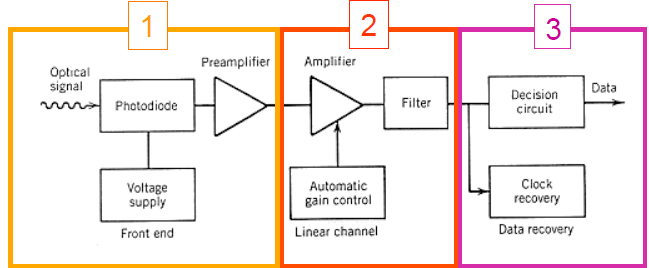
\includegraphics[scale=0.25]{ch5/image8}
\captionof{figure}{ }
\end{wrapfigure}
Les récepteurs sont composés de \textbf{trois} sections : le \textit{front-end} (détection (conversion
optique à électrique) et pré-amplification), le \textit{linear channel} (amplification et filtrage
du signal électrique (contrôle de l'maplitude et limitation du bruit)) et le \textit{data recovery} 
(circuit de décision).

\subsection{Front end}
Le but ici est de générer une tension signal $V_0$ à partir du photo-courant $I_p$ à l'aide d'une
résistance de charge $R_L$ et d'un pré-amplifier. Comme d'habitude il faut faire un choix : 
grande sensibilité (grand $R_L$) ou grande bande passante (petit $R_L$). Il existe deux front end
design
\begin{description}
\item[A grande impédance ($R_L\gg1$)] La résistance de charge est en parallèle avec la photodiode et
la différence de tension est amplifiée par l'AOP de gain $A$. La tension en sortie vaut donc 
$V_0=AR_LI_p$ à basse fréquence. On peut modifier l'effet capacitif (une photodiode $p-i-n$ c'est
un isolant et deux conducteurs, donc une capacité) par le placement d'une capacité qui tient donc 
compte des effets de charge et de décharge. Notons que la résistance d'entrée de l'AOP est supposée
infinie, la photodiode "verra" $R_L$. Donc
\begin{equation}
Z_i = \dfrac{R_L}{1+j\omega CR_L}\qquad\Rightarrow\qquad {V_0} = \frac{{A{R_L}}}{{1 + j\omega C{R_L}}}{I_p}
\end{equation}
La bande passante vaut alors
\begin{equation}
BW_1 = \dfrac{1}{R_LC}
\end{equation}
On retrouve bien le fait qu'une grande résistance d'entrée donne une grande sensibilité au récepteur
mais limite aussi sa bande passante.
\begin{center}
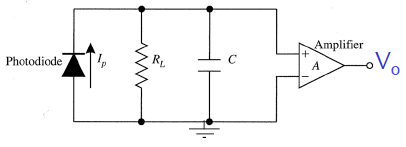
\includegraphics[scale=0.5]{ch5/image9}
\captionof{figure}{ }
\end{center}

\item[A transimpédance] Ceci permet de régler quelques limitations du circuit à grande impédance. 
\begin{equation}
{V_0} = \frac{{A{R_L}}}{{j\omega C{R_L} - (A - 1)}}{I_p}
\end{equation}
La bande passante vaut ici
\begin{equation}
BW = \dfrac{A-1}{R_LC}
\end{equation}
Grâce au gain $A$ de l'AOP, on peut avoir un grand gain et une grande bande passante en même temps. 
On parvient aussi à avoir un bruit faible avec ce montage (voir section 5.4.2).
\begin{center}
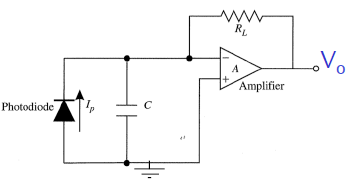
\includegraphics[scale=0.5]{ch5/image10}
\captionof{figure}{ }
\end{center}
\end{description}

\subsection{Linear amplification channel}
Le chaîne d'amplification linéaire se compose d'un amplificateur à grand gain (contrôlé 
automatiquement) et d'un filtre passe bas. On utilise celui-ci pour obtenir l'amplitude moyenne
souhaitée et on ajoute son gain automatiquement pour que ceci soit toujours le cas. \\

Le filtre passe bas de bande passante $\Delta f$ sert à limiter le bruit (électrique et/ou optique 
ainsi que celui du détecteur). Il doit être adapté selon la bande passante du signal 
transmis\footnote{Une bande passante trop basse élargi le pulse sur un temps supérieur au temps bit
et trop grand il y a trop de bruit et donc trop d'erreurs.}. Une fois de plus, il y a un compromis
entre l'efficacité du filtre et la bande passante. En pratique, il faut prendre $\Delta f \approx B$.

\subsection{Data-recovery section}
Le circuit de décision est la dernière partie du récepteur. Il doit comparer le niveau du signal
reçu à un seuil de décision pour fournir un débit binaire (voir diagrammes de l'œil). La 
synchronisation de celui-ci est importante. 

\subsubsection{Spectral density of a pseudo-random bit sequence}
Considérons une modulation OOK (RZ ou NRZ (si $T_B=T_0$). Soit la densité spectrale d'une séquence 
de bits aléatoires (Théorème de Wiener-Khinchin)
\begin{equation}
\tilde S(\omega ) = \frac{{{{\left| {\tilde A(\omega )} \right|}^2}}}{{4{T_B}}}(1 + \frac{{2\pi }}{{{T_B}}}\sum\limits_{k =  - \infty }^{ + \infty } {\delta [\omega  - k\frac{{2\pi }}{{{T_B}}}]} )
\end{equation}

\newpage
\begin{wrapfigure}[11]{r}{7cm}
%\vspace{-5mm}
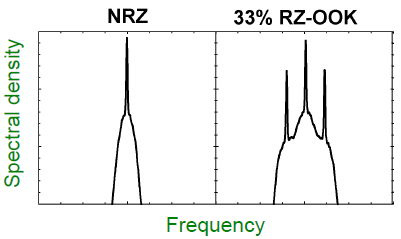
\includegraphics[scale=0.65]{ch5/image11}
\captionof{figure}{ }
\end{wrapfigure}
On retrouve le spectre du signal multiplié par 1 plus un peigne de fonction de Dirac. Si la forme
du pulse est un signal carré, on peut montrer que la densité spectrale présente un pic à la fréquence
$f=B$. Comme la TF d'un rectangle est une sinc, on va retrouver des pics à cause de ses zéros. \\

Le problème, pour les NRZ pseudo-aléatoires, c'est que le premier zéro de la transformée de Fourier 
de l'impulsion coïncide exactement avec la composante du peigne de Dirac et l'annule ainsi dans le
spectre du signal. Par contre, si le signal est filtré par un circuit de détection de bord, le signal correspondra à nouveau à un signal RZ pseudo-aléatoire avec un débit binaire de $2B$. La mesure du spectre de ce signal filtré fournit donc la valeur $f = 2B$.

\section{Noise mechanisms leading to current fluctuations in optical receivers: Shot noise and Thermal noise}
En pratique, même si $P_{in}$ est constant, le photo-courant $I(t)$ présente des fluctuations 
générées par le récepteur
\begin{equation}
I(t) = I_p + I_{dark} + i(t)
\end{equation}
où
\begin{description}
\item[Photo-courant moyen]
\begin{equation}
I_p = RP_{in}
\end{equation}

\begin{center}
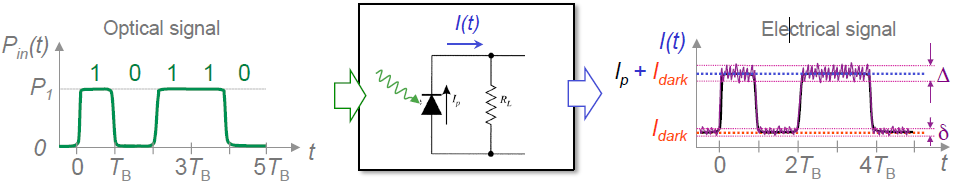
\includegraphics[scale=0.5]{ch5/image12}
\captionof{figure}{ }
\end{center}
\item[Courant noir] Il s'agit du courant moyen lorsque $P_{in}=0$, il est causé par le bruit thermique
(résistance $R_L$, sa tension varie au cours du temps) des porteurs libres. Il est généralement
négligeable face au photo-courant. 
\item[Fluctuations du courant] Il s'agit de processus stationnaires aléatoires qui ont une moyenne
nulle. On distincte deux contributions
\begin{enumerate}
\item Le \textit{shot-noise} (bruit de grenaille) lié à la quantification des particules. Lorsqu'on
détecte des photons sur un laps de temps, leur nombre n'est pas toujours identique : fluctuation
statistique du nombre de photon par unité de temps, même à puissance constante. On parle de 
"granulosité" dans le signal.
\item Le bruit thermique (ou de Nyquist). Si l'on mesure la tension d'une résistance dans laquelle
les charges bougent, on va voir des fluctuations liées au mouvement brownien des charges libres
dans un conducteur.
\end{enumerate}
\end{description}

\newpage
\subsection{Shot noise}
\begin{wrapfigure}[7]{r}{6cm}
\vspace{-8mm}
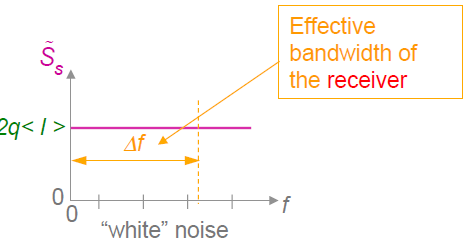
\includegraphics[scale=0.5]{ch5/image13}
\captionof{figure}{ }
\end{wrapfigure}
Le shot noise provient de la nature quantique de la lumière : fluctuation du nombre de photons
par unité de temps $N$ atteignant le détecteur et donc le nombre de porteurs libres générés. Ces
fluctuations obéissent à une statistique de Poisson $p(N)$ qui peut être approximée par une 
statistique Gaussienne (avec une certaine variance) pour un grand $\langle N\rangle$
\begin{equation}
I\left( t \right) = {I_p} + {i_s}\left( t \right)
\end{equation}
où $I_s$ est une distribution gaussienne. Avec le théorème de Wiener-Khinchin\footnote{La TF de 
la densité spectrale d'un signal est donné par la TF de l'auto-corrélation du signal. Ceci est 
utilisé dans les spectromètre à TF (donnant un très haute résolution).}, on peut obtenir
la densité spectrale du shot noise
\begin{equation}
{\tilde S_s}\left( f \right) = \int_{ - \infty }^{ + \infty } {\left\langle {{i_s}\left( t \right){i_s}\left( {t + \tau } \right)} \right\rangle {e^{ - j2\pi f\tau }}{\rm{d}}\tau } 
\end{equation}
où $\left\langle {{i_s}\left( t \right){i_s}\left( {t + \tau } \right)} \right\rangle  = \mathop {\lim }\limits_{T \to \infty } \frac{1}{{\Delta T}}\int\limits_{\Delta T} {{i_s}\left( t \right){i_s}\left( {t + \tau } \right)dt}$ est l'auto-corrélation de $i_s$. Ceci donne lieu à un \textit{bruit blanc} 
(indépendant de la fréquence) de la valeur vaut $2q<I>$.\\

On peut calculer la variance du shot noise
\begin{equation}
\sigma _s^2 = \left\langle {i_s^2\left( t \right)} \right\rangle  = 2q\left\langle I \right\rangle \Delta f
\end{equation}
où $\Delta f = \int_0^\infty  {{{\left| {\tilde H} \right|}^2}df}$. Comme le courant noir contribue
également au shot noise, on trouve finalement\\

\cadre{
\begin{equation}
\sigma _s^2 = 2q\left( {{I_p} + {I_{dark}}} \right)\Delta f
\end{equation}}\ \\


Comme la bande passante du détecteur $\Delta f$ es tlimitée par le filtre passe-bas, c'est lui 
qui contrôle la variance du bruit de grenaille : il est essentiel de filtrer dans le canal linéaire
pour limiter l'impact du bruit de grenaille. C'est pour cette raison que la bande passante du filtre
est prise proche de $B$ (en OOK).


\subsection{Thermal noise (also “Nyquist noise” or “Johnson noise”)}
Le bruit thermique provient des fluctuations de charge dans la résistance d'entrée $R_L$ à cause de 
l'agitation thermique aléatoire à la température $T$.
\begin{equation}
I(t) = I_p  + I_{dark} + I_T(t)
\end{equation}
où $I_T(t)$ est une distribution Gaussienne dont la densité spectrale est donnée par
\begin{equation}
{\tilde S_T}\left( f \right) = \int_{ - \infty }^{ + \infty } {\left\langle {{i_T}\left( t \right){i_T}\left( {t + \tau } \right)} \right\rangle {e^{ - j2\pi f\tau }}{\rm{d}}\tau } 
\end{equation}
On peut en déduire que la densité spectrale de bruit thermique vaut $4k_BT/R_L$ où $k_B$ est la 
constante de Boltzmann. Il s'agit encore une fois d'un bruit blanc. La variance du bruit thermique 
est donnée par
\begin{equation}
\sigma _T^2 = \left\langle {i_T^2\left( t \right)} \right\rangle  = \left( {\frac{{4{k_B}T}}{{{R_L}}}} \right)\Delta f
\end{equation}
\textbf{Attention}, les amplificateurs présents dans le récepteur génèrent aussi des fluctuations
thermiques : on en prend phénoménologiquement compte en multipliant le bruit thermique généré dans
la résistance de charge par le \textbf{amplifier noise figure $F_n$}. La variance thermique en \textit{front end} vaut alors
\begin{equation}
\sigma _T^2 \cong \left( {\frac{{4{k_B}T}}{{{R_L}}}} \right)\Delta f{F_n}
\end{equation}
Contrairement au bruit de grenaille, la variance du bruit thermique est indépendante de la puissance
optique d'entrée mais dépend de la température (on s'en doutait).

\subsection{Total variance of the noise}
Le shot noise et le bruit thermique sont deux processus indépendants avec des statistiques 
approximativement gaussiennes : on peut sommer les variances ${\sigma ^2} = \sigma _S^2 
+ \sigma _T^2$\footnote{$\sigma _{}^2 = \left\langle {{{\left( {I(t) - ({I_p} + {I_{dark}})} 
\right)}^2}} \right\rangle  = \left\langle {i_s^2\left( t \right) + i_T^2\left( t \right)} \right
\rangle  = \left\langle {i_s^2} \right\rangle  + \left\langle {i_T^2} \right\rangle$}. On en tire\\

\cadre{\begin{equation}
{\sigma ^2} = 2q\left( {{I_p} + {I_{dark}}} \right)\Delta f + \left( {\frac{{4{k_B}T}}{{{R_L}}}} \right){F_n}\Delta f
\end{equation}
où le shot noise dépend du courant moyen mais \textbf{pas} le thermal noise.}\ \\

\begin{wrapfigure}[11]{r}{8.5cm}
%\vspace{-5mm}
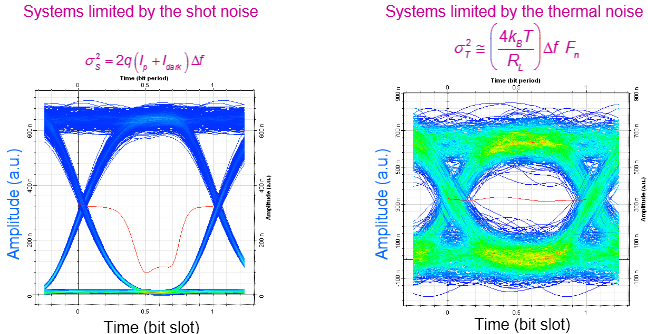
\includegraphics[scale=0.5]{ch5/image14}
\captionof{figure}{ }
\label{fig:id}
\end{wrapfigure}
Ceci montre qu'il est important de limiter la bande passante du récepteur $\Delta f$. La variance
$\sigma$ n'est rien autre que la valeur RMS du courant du bruit généré par le récepteur $p-i-n$. On
peut voir les différences entre ces deux bruit sur les diagrammes de l'œil. Ci-contre, on remarque
rapidement que le shot noise limite à gauche. En effet, celui-ci est proportionnel à $I_p$, les 
fluctuations sont plus importantes "en haut" du diagramme. Par contre, pour le bruit thermiques, 
elles sont importantes partout (à droite).

\section{Signal-to-noise ratio (SNR$_e$) of an optical detector}
Par définition, le SNR$_e$ d'un détecteur optique est le rapport entre la puissance électrique 
moyenne et la puissance électrique du bruit
\begin{equation}
SN{R_e} = \frac{{{I_p}^2}}{{\left\langle {{{\left( {I\left( t \right) - \left( {{I_p} + {I_{dark}}} \right)} \right)}^2}} \right\rangle }} = \frac{{{I_p}^2}}{{\sigma _S^2 + \sigma _T^2}}
\end{equation}
où $I_p = RP_{in}$. On utilisera le SNR$_e$ pour déterminer le taux d'erreur. Nous allons considérer
les récepteurs $p-i-n$ et APD séparément.

\subsection{$p-i-n$ receivers}
Le bruit vient du bruit de grenaille et du thermique. On en tire, en reprenant les précédentes
expressions
\begin{equation}
SN{R_e} = \frac{{{R^2}P_{in}^2}}{{2q\left( {R{P_{in}} + {I_{dark}}} \right)\Delta f + \left( {\frac{{4{k_B}T}}{{{R_L}}}} \right){F_n}\Delta f}}
\end{equation}
où $R= \eta q/(h\nu)$. Lorsque la contribution principale du SNR$_e$ est le bruit thermique
\begin{equation}
SN{R_e}^{Thermal} = \frac{{{R^2}P_{in}^2}}{{\underbrace{2q(RP_{in}+I_{dark})\Delta f}_{\ll}+ \left( {\frac{{4{k_B}T}}{{{R_L}}}} \right){F_n}\Delta f}} \cong \frac{{{R^2}P_{in}^2{R_L}}}{{4{k_B}T{F_n}\Delta f}}
\end{equation}
Le SNR$_e$ est amélioré (augmente) lorsque
\begin{enumerate}
\item $P_{in}$ et/ou $R_L$ augmentent ; un minimum de puissance est requis et il y a un compromis 
entre un grand SNR$_e$ et une grande bande passante.
\item $T$ et/ou $\Delta f$ sont réduits; importance du contrôle de la température et du filtre
passe-bas dans le récepteur (linear channel).
\end{enumerate}


\subsubsection{Noise equivalent power (NEP)}
On utilise parfois le NEP ($[W.Hz^{-1/2}]$) pour évaluer la puissance optique minimale nécessaire 
au détecteur pour une bande passante $\Delta f$ donnée. Par définition
\begin{equation}
NEP \buildrel \Delta \over = \frac{{P_{in}^{Th = 1}\left[ {{\rm{such as}}SN{R_e}^{Thermique} = 1} \right]}}{{\sqrt {\Delta f} }}
\end{equation}
où il convient d'utiliser $P_{in} = NEP\sqrt{\Delta f}$ avec $\Delta f$ la bande passante électrique
du \textbf{récepteur} !
\begin{equation}
NEP = {\left( {\frac{{4{k_B}T{F_n}}}{{{R^2}{R_L}}}} \right)^{{\raise0.7ex\hbox{$1$} \!\mathord{\left/
 {\vphantom {1 2}}\right.\kern-\nulldelimiterspace}
\!\lower0.7ex\hbox{$2$}}}} = \frac{{h\nu }}{{\eta q}}{\left( {\frac{{4{k_B}T{F_n}}}{{{R_L}}}} \right)^{{\raise0.7ex\hbox{$1$} \!\mathord{\left/
 {\vphantom {1 2}}\right.\kern-\nulldelimiterspace}
\!\lower0.7ex\hbox{$2$}}}}
\end{equation}\ \\

Lorsque la contribution principale du SNR$_e$ est le bruit thermique
\begin{equation}
SN{R_e}^{Shotnoise} = \frac{{{R^2}P_{in}^2}}{{2qR{P_{in}}\Delta f + \underbrace{\left(\frac{4k_BT}{R_L}\right)F_n\Delta f}_{\gg}}} \cong \frac{{\eta {P_{in}}}}{{2h\nu \Delta f}}
\end{equation}
Dans ce cas, le SNR$_e$ augmente lorsque
\begin{enumerate}
\item $P_{in}$ est augmentée ; une puissance minimale est nécessaire.
\item $\Delta f$ est diminuée ; importance du filtre passe-bas dans le récepteur (linear channel)
\end{enumerate}

On peut donner une relation entre le SNR$_e$ et le nombre de photons par bit $N_p^{bit}$
\begin{equation}
{P_{in}} = N_p^{bit}h\nu B\qquad\Rightarrow\qquad
SN{R_e}^{Shotnoise} = \frac{{\eta {P_{in}}}}{{2h\nu \Delta f}} \cong \frac{{\eta N_p^{bit}B}}{{2\Delta f}} \approx \eta N_p^{bit}
\end{equation}
On peut montrer qu'un SNR$_e$ de 20dB peut être atteint avec 100 photons par bits!


\subsection{APD based receivers}
Ici, le photo-courant est amplifié d'un facteur $M$ par rapport à celui de la photodiode 
$p-i-n$
\begin{equation}
I = {R_{{\rm{APD}}}}{P_{in}} = MR{P_{in}}
\end{equation}
Supposons que l'on ai juste un amplificateur sans bruit. La variance totale est alors donnée par
\begin{equation}
{\sigma ^2} = \left\langle {{{[M\;{i_s}(t)]}^2}} \right\rangle  + \left\langle {{i_T}{{(t)}^2}} \right\rangle  = 2q{M^2}\left( {R{P_{in}} + {I_{dark}}} \right)\Delta f + \left( {\frac{{4{k_B}T}}{{{R_L}}}} \right){F_n}\Delta f
\end{equation}
où $\Delta f$ est la bande passante électronique du récepteur. Le courant thermique est 
indépendant du mécanisme d'amplification (indépendant de $M$). Si le SNR$_e$ est dominé par 
le bruit thermique, on gagne un facteur $M^2$. Le SNR$_e$ n'est pas affecté si le récepteur
est limité par le shot noise\footnote{Erreur et thermal noise, non?}. \\

Cependant, dans les APD réels, l'amplification es tun processus aléatoire\footnote{Le nombre
d'électrons généré pour un photon varie.} qui va causer une contribution au bruit : \textbf{noisy
amplification}. On va modéliser ça en utilisant $F_a$ pour écrire la variance totale du shot noise
\begin{equation}
{\sigma _s}^2 = 2q{M^2}{F_A}\left( {R{P_{in}} + {I_{dark}}} \right)\Delta f
\end{equation}
où $F_a$ est l'\textbf{excess noise factor}. Par définition
\begin{equation}
{F_a} \buildrel \Delta \over = \left\langle {{m^2}} \right\rangle /{M^2} = {k_a}M + (1 - {k_a})(2 - 1/M)
\end{equation}
où $\langle m \rangle = M$. Nous faisons ici l'hypothèse que seuls les électrons sont injectés dans
la couche d'amplification. En effet
\begin{equation}
k_a \ll 1 \quad\to \quad F_a<2\qquad\text{et}\qquad k_a\approx1\quad\to\quad F_a\approx M
\end{equation}
La condition de droite signifie que les électrons \textbf{et} les trous participent ce qui crée
un bruit associé très élevé (car, en général, $M>2$). Ceci justifie pourquoi on utilise l'un où
l'autre pour les meilleures performances ($\alpha_h \ll \alpha_e$ ou $\alpha_e \ll \alpha_h$). En
conclusion, pour les récepteurs basés sur APD, la puissance moyenne du signal est multipliée par
$M^2$, la variance du bruit de tir est multipliée par $M^2F_a$ et la variance du bruit thermique 
n'est pas affectée.\\

\begin{wrapfigure}[10]{r}{6.5cm}
\vspace{-7mm}
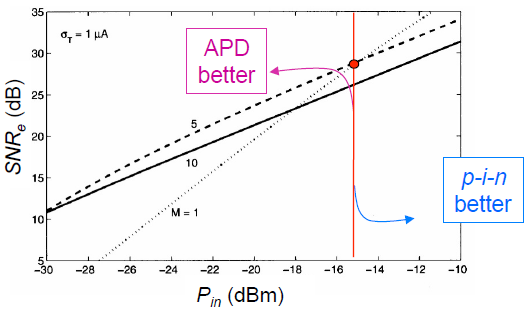
\includegraphics[scale=0.5]{ch5/image15}
\captionof{figure}{$M=1$ pour la photodiode $p-i-n$ car pas d'amplification}
\end{wrapfigure}
Si le récepteur est limité par le shot noise
\begin{equation}
SN{R_e} = \frac{{{{(R{P_{in}})}^2}}}{{2q{F_a}\left( {R{P_{in}} + {I_{dark}}} \right)\Delta f}}
\end{equation}
La photodiode en avalanche  augmente le courant, mais dégrade le SNR$_e$ par rapport au récepteurs
$p-i-n$ d'un facteur $F_a$ ! Dans le cas général pour les APD
\begin{equation}
SN{R_e} = \frac{{{{(MR{P_{in}})}^2}}}{{2q{M^2}{F_a}\left( {R{P_{in}} + {I_{dark}}} \right)\Delta f + \left( {\frac{{4{k_B}T}}{{{R_L}}}} \right){F_n}\Delta f}}
\end{equation}
\textbf{Les APD sont attractifs lorsque le bruit thermique domine le shot noise} !
\begin{center}
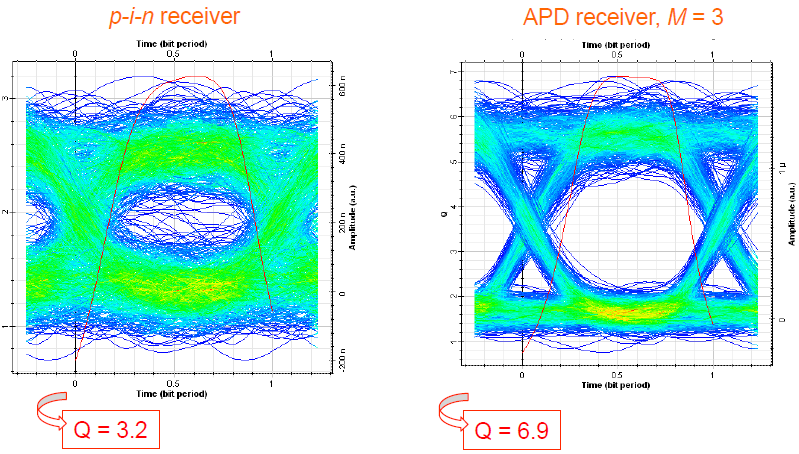
\includegraphics[scale=0.4]{ch5/image16}
\captionof{figure}{$P_{in}=-37$ dBm, NRZ. Ici, l'ADP est préférable.}
\end{center}

\newpage
\section{Receiver sensitivity and Bit-Error Rate (BER)}
\begin{wrapfigure}[9]{l}{11cm}
\vspace{-7mm}
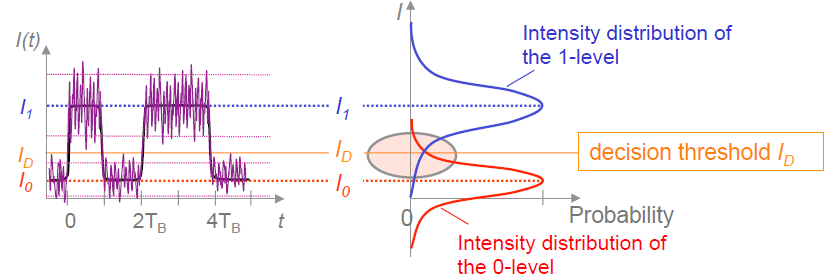
\includegraphics[scale=0.5]{ch5/image17}
\captionof{figure}{ }
\end{wrapfigure}
Un récepteur est plus sensible lorsqu'il atteint les mêmes performances pour une puissance incidente
plus faible. Pour la définir, il faut savoir mesurer la performance d'un récepteur : c'est le nombre
de fois qu'il ne se trompe pas pour une certaine quantité de bit reçus, soit l'erreur binaire.\\

Le \textbf{Bit-Error-Rate (BER)} est la probabilité qu'une erreur ai lieu dans l'identification d'un
bit par le récepteur. A cause du bruit (même si le signal est sans bruit, l'amplification en 
introduit) causant des fluctuations, des erreurs sont possibles.\\

\begin{wrapfigure}[9]{r}{5cm}
\vspace{-9mm}
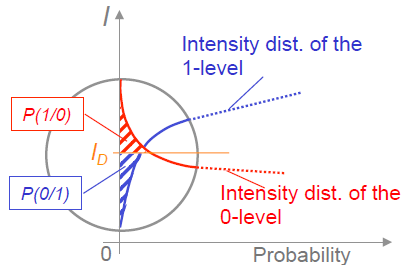
\includegraphics[scale=0.5]{ch5/image18}
\captionof{figure}{ }
\end{wrapfigure}

Posons
\begin{itemize}
\item[$\bullet$] $p(1)$ la probabilité de recevoir un bit '1'
\item[$\bullet$] $p(0)$ la probabilité de recevoir un bit '0'
\item[$\bullet$] $P(0/1)$ la probabilité de déduire '1' lorsque '0' est reçu
\item[$\bullet$] $P(1/0)$ la probabilité de déduire '0' lorsque '1' est reçu
\end{itemize}\ \\

Le BER est alors donnée par
\begin{equation}
BER = p\left( 1 \right)P\left( {0/1} \right) + p\left( 0 \right)P\left( {1/0} \right) = \frac{1}{2}\left[ {P\left( {0/1} \right) + P\left( {1/0} \right)} \right]
\end{equation}
C'est la probabilité d'avoir '1' multiplié par la probabilité d'interpréter '1' comme '0' + \dots Nous
avons ici fait l'hypothèse que $p(0)=p(1)=1/2$ car il n'y a pas de raison d'avoir plus de '1' que
de '0' dans un signal. On peut calculer les probabilités conditionnelles
\begin{equation}
P\left( {0/1} \right) = \frac{1}{{{\sigma _1}\sqrt {2\pi } }}\int_{ - \infty }^{{I_D}} {\exp \left[ { - \frac{{{{\left( {I - {I_1}} \right)}^2}}}{{2\sigma _1^2}}} \right]dI}  = \frac{1}{2}erfc\left( {\frac{{{I_1} - {I_D}}}{{{\sigma _1}\sqrt 2 }}} \right)
\end{equation}
\begin{equation}
P\left( {1/0} \right) = \frac{1}{{{\sigma _0}\sqrt {2\pi } }}\int_{{I_D}}^{ + \infty } {\exp \left[ { - \frac{{{{\left( {I - {I_0}} \right)}^2}}}{{2\sigma _0^2}}} \right]dI}  = \frac{1}{2}erfc\left( {\frac{{{I_D} - {I_0}}}{{{\sigma _0}\sqrt 2 }}} \right)
\end{equation}
Ces deux probabilités dépendent de $I_D$, le courant de décision où erfc est la fonction 
d'erreur complémentaire. Le BER s'écrit alors
\begin{equation}
BER = \frac{1}{4}\left[ {erfc\left( {\frac{{{I_1} - {I_D}}}{{{\sigma _1}\sqrt 2 }}} \right) + erfc\left( {\frac{{{I_D} - {I_0}}}{{{\sigma _0}\sqrt 2 }}} \right)} \right]
\end{equation}
Comme il dépend bien évidemment aussi de $I_D$, nous allons chercher la valeur $I_D^*$ qui 
le minimise
\begin{equation}
\frac{{{I_1} - I_D^*}}{{{\sigma _1}}} = \frac{{I_D^* - {I_0}}}{{{\sigma _0}}} = Q\qquad\Rightarrow
\qquad I_D^* = \frac{{{\sigma _0}{I_1} + {\sigma _1}{I_0}}}{{{\sigma _0} + {\sigma _1}}}
\end{equation}
Celui-ci est tracé en rouge à la \autoref{fig:id}. Par définition, le \textbf{facteur de qualité} 
$Q$ du signal reçu est donné par
\begin{equation}
Q \buildrel \Delta \over = \frac{{{I_1} - {I_0}}}{{{\sigma _0} + {\sigma _1}}}
\end{equation}
Il s'agit du rapport de la différence entre les photo courants sur la somme RMS des fluctuations
du courant. \\

Lorsque le bruit du récepteur est dominé par le thermique, $\sigma_0=\sigma_1 \Rightarrow 
I_D^{*Thermal} = \frac{{{I_1} + {I_0}}}{2}$ : les valeurs moyennes du courant des niveaux '1' et '0'
sont équidistantes du seuil de décision optimal.\\

La valeur optimale du BER vaut
\begin{equation}
BER* = BER({I_D}*) = \frac{1}{2}erfc\left( {\frac{{{I_1} - {I_0}}}{{\sqrt 2 \left[ {{\sigma _1} + {\sigma _0}} \right]}}} \right) = \frac{1}{2}erfc\left( {\frac{Q}{{\sqrt 2 }}} \right) \cong \frac{{\exp \left( { - \frac{{{Q^2}}}{2}} \right)}}{{Q\sqrt {2\pi } }}
\end{equation}\ 

\begin{wrapfigure}[9]{l}{7cm}
\vspace{-9mm}
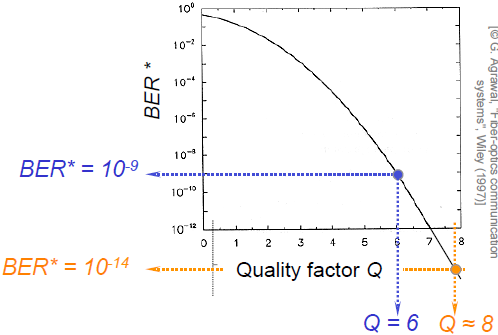
\includegraphics[scale=0.5]{ch5/image19}
\captionof{figure}{ }
\end{wrapfigure}
En faisant l'hypothèse raisonnable que $Q\geq 3$. Il y a donc une relation simple entre le 
$BER^*$ et $Q$ : lorsque $Q$ augmente, le $BER$ diminue rapidement(d'où le nom \textit{facteur de 
qualité}). Lorsque $Q=0$, on a une chance sur deux de se tromper ('1' ou '0').\\
\ \\
\ \\

\subsubsection{Sensibilité du détecteur}
Supposons que le seuil de décision est optimal ($I_D=I_D^*$). La \textbf{sensibilité du détecteur} 
est la puissance optique moyenne minimale incidente $\bar{P_{rec}}$ nécessaire à un récepteur 
pour avoir un BER < $10^{-9}$ ($Q=6$).\\

Faisons trois hypothèses
\begin{enumerate}
\item Le format de modulation est NRZ
\item La puissance optique moyenne dans l'état \textit{off} $P_0$ est nulle
\item Le courant noir $I_{dark}$ peut être négligé
\end{enumerate}
La dérivation est donnée au \textit{slide 36}. L'idée est d'écrire la puissance moyenne du signal
en fonction de $Q$ puis d'inverser la relation. On trouve alors\\

\cadre{
\begin{equation}
\overline {{P_{rec}}}  = \frac{Q}{R}\left( {Qq\Delta f + {\sigma _T}} \right) = \frac{Q}{R}\left( {Qq\Delta f + {{\left( {\frac{{4{k_B}T}}{{{R_L}}}} \right)}^{1/2}}\Delta {f^{1/2}}F_n^{1/2}} \right)
\end{equation}}\ \\

Il s'agit de la puissance nécessaire au récepteur pour avoir une certaine valeur de $Q$ (qui permet
de remonter au BER). La sensibilité d'un récepteur $p-i-n$ a donc une contribution venant du 
shot noise (premier terme, celui proportionnel à $\Delta f$ et à la charge élémentaire $q$) et une venant du bruit thermique (le second terme, celui proportionnel à $\Delta f^{1/2}$ et à $k_BT$).
\newpage
\section{Degradation of the receiver sensitivity \& Power penalty}
Jusqu'ici nous avons considéré un signal idéal : tous les pulses '1' avaient la même énergie et le
même profil temporel et les pulses '0' n'avaient pas d'énergie. Seul le bruit du récepteur était
pris en compte. Hélas, le transmetteur génère aussi du bruit, certains bruits générés par les
amplificateurs sont inévitables, la forme des pulses n'est pas parfaite et il y a des distorsions
du signal.\\

Pour maintenir $Q$, il faut augmenter la puissance optique moyenne qui atteint le détecteur. On 
utilise alors la \textbf{power penality}. C'est l'augmentation de puissance nécessaire au récepteur
pour outrepasser la dégradation causée par des conditions non-idéales.\\

Les sources de pénalité de puissances sont liées à deux propriétés non idéale du 
\textbf{transmetteur} (Hyp. : les sources de pénalité de la propagation du signal sont ignorées)
\begin{enumerate}
\item L'énergie portée par les '0'
\item Le bruit en intensité
\end{enumerate}

\subsection{Penalty due to average optical power $P_0$ carried by the '0' bits}
L'origine de l'énergie présente au bit '0' dépend de la modulation. 
\begin{description}
\item[Modulation directe] Allumer un laser demande un certain seuil, il faut du délai. Pour moduler
plus rapidement, on se met un peu au dessus de ce seuil pour éviter le délai de démarrage. 
\item[Modulation indirecte] Utilise un Mach-Zehnder dont les interférences destructives ne le sont
jamais totalement.
\end{description}
Pour s'en sortie, on utilise le \textbf{rapport d'extinction} $r_{ex}$ comme le rapport entre la
puissance optique moyenne $P_1$ et la sortie du transmetteur
\begin{equation}
{r_{ex}} \buildrel \Delta \over = \frac{{{P_0}}}{{{P_1}}}
\end{equation}
La puissance moyenne reçue est-elle une fonction de $Q$ et $r_{ex}$ ? L'idée est la même que 
précédemment : on exprime $Q$ comme une fonction de $P$ et on l'inverse. Hélas, la pénalité de 
puissance causée par $r_{ex}$ ne se calcule pas facilement à cause de la dépendance en puissance du
shot noise (détail \textit{slide 40})
\begin{equation}
Q = \frac{{2R\overline {{P_{rec}}} }}{{{\sigma _1} + {\sigma _0}}}\frac{{\left( {1 - {r_{ex}}} \right)}}{{\left( {1 + {r_{ex}}} \right)}}
\end{equation}
où $\sigma  = {\sigma _T} + {\sigma _s}(\overline {{P_{rec}}} )$. En faisant l'hypothèse que 
le bruit du récepteur est dominé par le bruit thermique (${\sigma _1} = {\sigma _0} = {\sigma _T}$), 
on en tire
\begin{equation}
Q = \frac{{R\overline {{P_{rec}}} }}{{{\sigma _T}}}\frac{{\left( {1 - {r_{ex}}} \right)}}{{\left( {1 + {r_{ex}}} \right)}}\qquad\Rightarrow\qquad \overline {{P_{rec}}} \left( {{r_{ex}}} \right) = \frac{{\left( {1 + {r_{ex}}} \right)}}{{\left( {1 - {r_{ex}}} \right)}}\frac{{Q{\sigma _T}}}{R}
\end{equation}
La pénalité vaut donc
\begin{equation}
Penalty = \frac{{\overline {{P_{rec}}} \left( {{r_{ex}}} \right)}}{{\overline {{P_{rec}}} \left( {{r_{ex}} = 0} \right)}} = \frac{{\left( {1 + {r_{ex}}} \right)}}{{\left( {1 - {r_{ex}}} \right)}}
\end{equation}
\newpage

\begin{wrapfigure}[10]{l}{6cm}
%\vspace{-9mm}
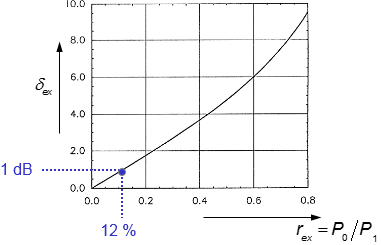
\includegraphics[scale=0.6]{ch5/image20}
\captionof{figure}{ }
\end{wrapfigure}
Celle-ci augmente de façon monotone avec $r_{ex}$ est dépend de $Q$. On définit ${\delta _{ex}} 
= 10{\log _{10}}\left( {Penalty} \right)$ comme la pénalité en dB. De cette façon
\begin{equation}
{\delta _{ex}} = 10{\log _{10}}\frac{{\left( {1 + {r_{ex}}} \right)}}{{\left( {1 - {r_{ex}}} \right)}}
\end{equation}
La figure ci-contre montre l'évolution de la pénalité en puissance (échelle dB) comme une fonction 
de $r_{ex}$. La pénalité est de 1 dB lorsque $r_{ex}=0.12$. Dans les modulateurs $MZ$, le rapport
d'extinction vaut à peu près -20 dB ; on peut négliger le pénalité de puissance due à l'énergie 
présente dans le '0' dans ces systèmes. 


\subsection{Penalty due to the intensity noise of the transmitter}
Pour la simplicité, considérons une approche phénoménologique en considérant un terme additionnel
dans la variance du bruit (on suppose les sources indépendantes)
\begin{equation}
{\sigma ^2} = \sigma _S^2 + \sigma _T^2 + \sigma _I^2
\end{equation}
Le bruit du signal peut venir du bruit du laser (bruit d'intensité du transmetteur) ou par celui
généré dans l'amplificateur. On se concentrera ici sur la première option. L'écart type est donné
par
\begin{equation}
{\sigma _I} = R{\left\langle {\left( {\Delta P_{in}^2} \right)} \right\rangle ^{{1 \mathord{\left/
 {\vphantom {1 2}} \right.
 \kern-\nulldelimiterspace} 2}}} = R{P_{in}}{r_l}
\end{equation}
où nous avons introduit (pour des raisons pratiques) le coefficient $r_l$\footnote{Sachant que $\frac{1}{{SN{R_o}}} = \frac{{{{\left\langle {\left( {\Delta P_{in}^2} \right)} \right\rangle }^{{1 \mathord{\left/
 {\vphantom {1 2}} \right.
 \kern-\nulldelimiterspace} 2}}}}}{{{P_{in}}}} \buildrel \Delta \over = {r_I}$}. Le \textit{slide 42}
 donne le facteur de qualité
 \begin{equation}
[Q = \frac{{2R\overline {{P_{rec}}} }}{{{{\left( {\sigma _S^2 + \sigma _T^2 + \sigma _I^2} \right)}^{{1 \mathord{\left/
 {\vphantom {1 2}} \right.
 \kern-\nulldelimiterspace} 2}}} + {\sigma _T}}}
 \end{equation}
Qui doit être inversé. Le \textit{slide 43} donne le détail mathématique. On y trouve la puissance
optique moyenne au récepteur
\begin{equation}
\overline {{P_{rec}}}  = \frac{{q\Delta f{Q^2} + {\sigma _T}Q}}{{R\left( {1 - r_l^2{Q^2}} \right)}}
\end{equation}
Ce qui donne comme pénalité
\begin{equation}
Penalty = \frac{{\overline {{P_{rec}}} \left( {{r_l}} \right)}}{{\overline {{P_{rec}}} \left( {{r_l} = 0} \right)}} = \frac{1}{{\left( {1 - r_l^2{Q^2}} \right)}}
\end{equation}

\begin{wrapfigure}[11]{l}{6cm}
\vspace{-5mm}
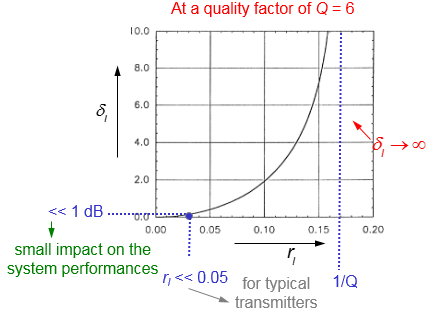
\includegraphics[scale=0.5]{ch5/image21}
\captionof{figure}{ }
\end{wrapfigure}
Contrairement au cas précédent, la pénalité en puissance dépend de $Q$ lorsque le bruit d'intensité 
du laser est considéré. Ceci vient du fait que les variation en amplitude du courant augmente 
avec la puissance moyenne puisqu'une partie de ces fluctuations provient du laser lui-même. En 
définissant ${\delta _l} =  - 10{\log _{10}}\left( {1 - r_l^2{Q^2}} \right)$, on voit bien que
celui-ci dépend du facteur de qualité $Q$. La pénalité tend vers l'infini lorsque $r_l\to 1/Q$, 
c'est-à-dire lorsque SNR$_o\to Q$. Sans tenir compte des pénalité, le SNR$_o$ limite intrinsèquement
le facteur $Q$ réalisable. Pour un système de télécom à $Q=6$, il faut que SNR$_o>6$.

\newpage
\section{Qualitative measurement of the performances of a $p-i-n$ receiver: Estimation/measurement of the BER at different power levels }
Pour mesurer la sensibilité ou le pénalité de puissance, le bruit, ... il faut mesurer les 
performances du système.  La méthode est simple
\begin{enumerate}
\item On envoie une séquence de bits pseudo-aléatoire dans le système
\item On compare la séquence en sortie avec la séquence originale pour évaluer le BER.
\end{enumerate}
Ceci peut être fait pour différentes puissances d'entrées et différentes longueurs de propagation. 
Le BER nous donne ainsi toutes les informations. Un exemple est donné au \textit{slide 46}.